\subsection{Phase I\label{sec:phaseI}}

Phase I presents a simple and functional cross-layer solution to enable a transfer system between all major DeFi ecosystems. It is a PoC with enforced limited functionality to demonstrate the capability of the system.

The main actors in this phase are: an L1 vault in charge of redistributing liquidity, dedicated vaults on each L2, users engaging and providing the required liquidity and a relayer in charge of communicating the different supported networks. All the actors and their interactions are depicted on Fig.~(\ref{fig:v1_mosaic}).

\begin{figure}[h]
    \centering
    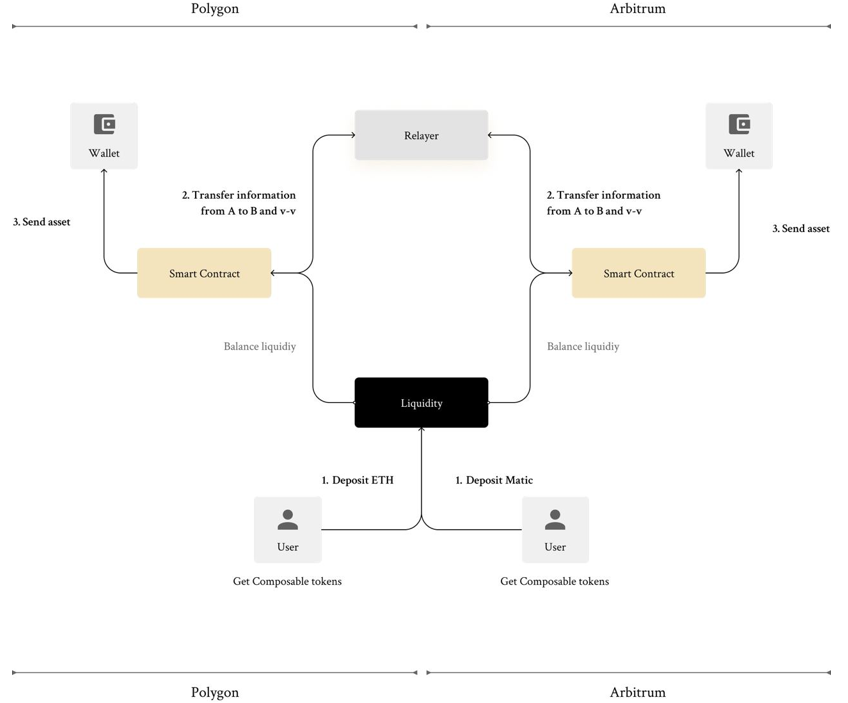
\includegraphics[width=1\textwidth]{images/mosaic/v1.png}
    \caption{Polygon-Arbitrum transfer scheme in Mosaic v1.}
    \label{fig:v1_mosaic}
\end{figure}

As you can see on Fig.~(\ref{fig:v1_mosaic}), a transfer consists of 2 important events: the lock event that happens on the source layer and the release event that is triggered by our relayer system on the destination one. This interaction is done on the L2Vault contract, with the lock happening using the \textit{depositERC20} method, while for the asset release, the \textit{withdrawTo} method is called on the L2Vault contract deployed on the other side.

In terms of the necessary liquidity for these actions to happen, users deposit liquidity using the VaultL1 smart contract deployed on L1 mainnet. Users obtain rewards in form of LAYR tokens in exchange for providing liquidity. L1 Vault acts as master with regards the L2 vaults, and redistributes the liquidity on demand. 

By leveraging a lock/unlock pattern on phase I, we were able to proof that interoperability can be obtained in the DeFi space, and that a single curated interface is enough for the user to operate on different layers and chains. We also obtained data about the  user experience and liquidity demands on different networks. Nevertheless, we kept the functionality limited for testing purposes. Thus, we dedicate next phase to enhance and open the protocol to more complex features.